\documentclass[runningheads]{llncs}
\usepackage{graphicx}
\usepackage[width=122mm,left=12mm,paperwidth=146mm,height=193mm,top=12mm,paperheight=217mm]{geometry}
\usepackage{amsmath,amssymb} % define this before the line numbering.

\DeclareMathOperator*{\argmin}{argmin}

%\usepackage{ruler}
\usepackage{color}

%\documentclass{llncs}
%\usepackage{graphicx}
%\usepackage{geometry}
%\geometry{margin=2cm}
%\usepackage{amsmath}

\usepackage{pgfplots}
\usepackage{filecontents}
\usepackage[caption=false]{subfig}
\usepackage{listings}
\lstset{
basicstyle=\small\ttfamily,
columns=flexible,
breaklines=true
}

\begin{document}
\title{Dissecting Neural Style Transfer}
\author{Xi Du}
\institute{Australian National University, Australia\\
\email{u6559090@anu.edu.au}}
\maketitle 
\begin{abstract}
\cite{method}

\keywords{Neural network, Deep learning, 
Small data, Interpretability .}
\end{abstract}

\section{Introduction}

\section{Literature Review}

\section{Method}

\subsection{Deep Neural Network}

For the purpose of implementing and even extending neural style transfer algorithms,
it is not necessary to understand how a neural network is trained, because
we can use pretrained model for example vgg19 \cite{vgg19}.

It is necessary to point out that a deep neural network that neural style transfer
is concerend about
is just a sequence of functions
$F_1,F_2,F_3,...$
whose inputs and outputs are all multi-dimensional arrays, as illustrated in Figure \ref{f1f2f3}.
\begin{figure}
\center
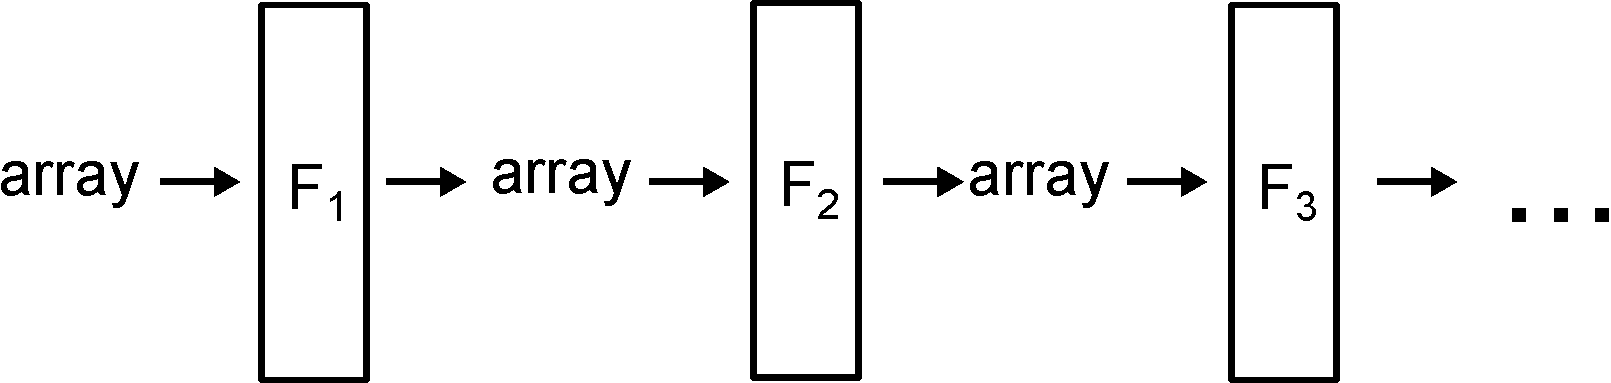
\includegraphics[width=0.6\textwidth]{f1f2f3.pdf}
\caption{A deep neural network \label{f1f2f3}}
\end{figure}
Because the arrays have usually more than two numbers of dimensions
they are not really matrices.
The arrays are called tensors (as in TensorFlow or torch.Tensor in PyTorch) 
but actual tensor algebra in a mathematical sense is rarely relevant.
The functions need to be differentiable, which is handled automatically by modern 
deep learning frameworks.
Other than that we can treat the functions as blackboxes because we are 
not concerned of training the model.
A ``layer'' in a deep neural network refers to a few consecutive functions together.
It is not particularly necessary to consider ``layers'' in this work. 
Though it is important to note that in our illustrations there are functions instead of layers.

\subsection{vgg19 model}
For the vgg19 model that most neural style transfer implementations available are based on,
The inputs and outpus of each function are all arrays with 4 dimensions.
The word ``dimension'' here may mean something slightly different from what ``dimension'' means in
for example ``$3$-dimension vector''. 
Some people call the number of dimensions ``rank'' which would then raise another confusion with the rank of matrices.
We give an illustration for the vgg19 model in Figure \ref{vgg512}
\begin{figure}
\center
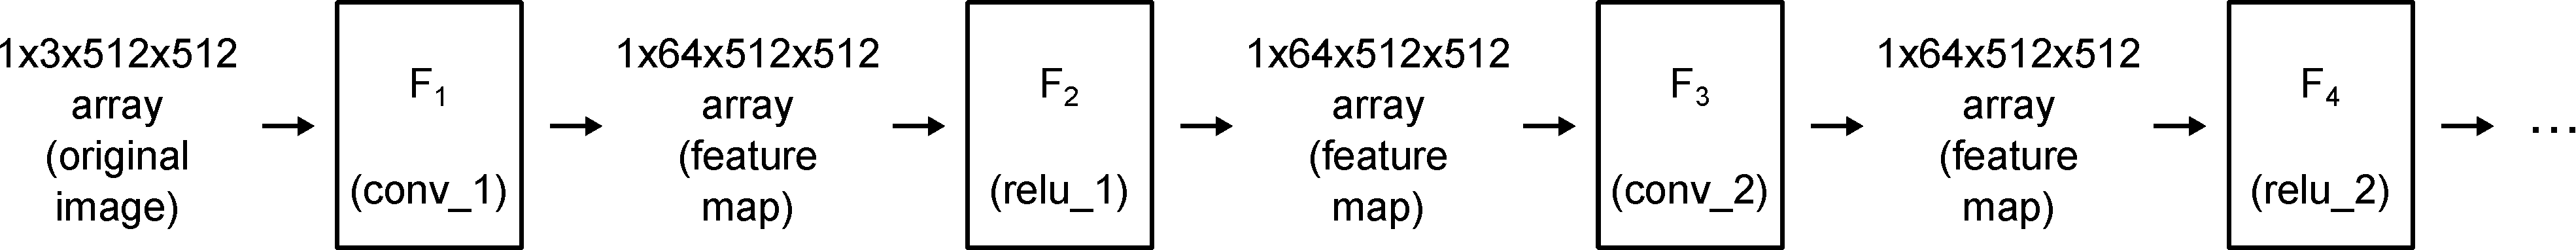
\includegraphics[width=\textwidth]{vgg512.pdf}
\caption{The VGG19 model with an $512\times512$ RGB image as its input \label{vgg512}}
\end{figure}

The 1st dimension is the ``batch'' dimension, which means that you can put several images through the
series of functions.
In neural style transfer implementations it is usually just one image each time.
So the 1st dimension is always 1, even between the $F$ functions, throughout this work.

The 2nd dimension is the ``feature'' dimension. For a raw RGB image, it is 3.
Intermediate arrays between, for example, $F_3$ and $F_4$, usually 
have a size much larger than 3, such as 64 or 128.

The 3nd and 4th dimensions are just spatial locations. 
For a $512\times512$ image they are 512 and 512. 
For intermediate arrays, these 2 dimensions are sometimes scaled down
to half or even $\frac{1}{4}$ of the sizes of the image.

The functions $F_1,F_2,F_3,...$ now have meaningful names such as relu\_1, conv\_2 now.
[Not actually necessary to know but insert your elaborations here]

The arrays after the initial image are called feature maps, because their value means
``how much a feature x exists at position y and x''.
For example in a $1\times64\times512\times512$ feature map, it means there are 64 types of features.
and its [1, 17, 111, 222] element, would then refer to the extent that the 17th type feature exists
at the position of the 222th column of the 111th row. This ``extent'' could also be negative.

\subsection{Vanilla neural style transfer}

The vanillay neural style transfer algorithm \cite{nst} is 
structured as iteratively solving an optimisation problem.
The argument to optimise is the image as a multidimensional array,
of size $1\times3\times512\times512$ for example.
The interative solver can be many, but in our case it is 
L-BFGS [Maybe elaborate on L-BFGS here]. 
The initial value of the argument could be either white noise or the content image,
but the latter appeared to make the optimisation much easier.

The key issue here is still how to structure the optimisation target.
The value to minimise is a linear combination of a ``style loss'' 
and ``content loss''.
Although these appeared to be two weights,
actually only their ratio mattered.
We simply fixed the weight of the content loss to 1 and
leave the weight of the style loss as a adjustable hyperparameter $k$.
\begin{align}
\argmin\limits_{\text{image}} (kL_\text{style}+L_\text{content})
\end{align}

The content loss is the easier one to explain of the two losses.
It is the mean square error between the outputs of a certain function in the
vgg19 taking the current argument image and the content image as inputs respectively.
We say ``a certain'' function because the output of which function to choose is
adjustable.
A typical choice is the output of \verb|conv_4| function. See Figure \ref{contentloss}.
\begin{figure}
\center
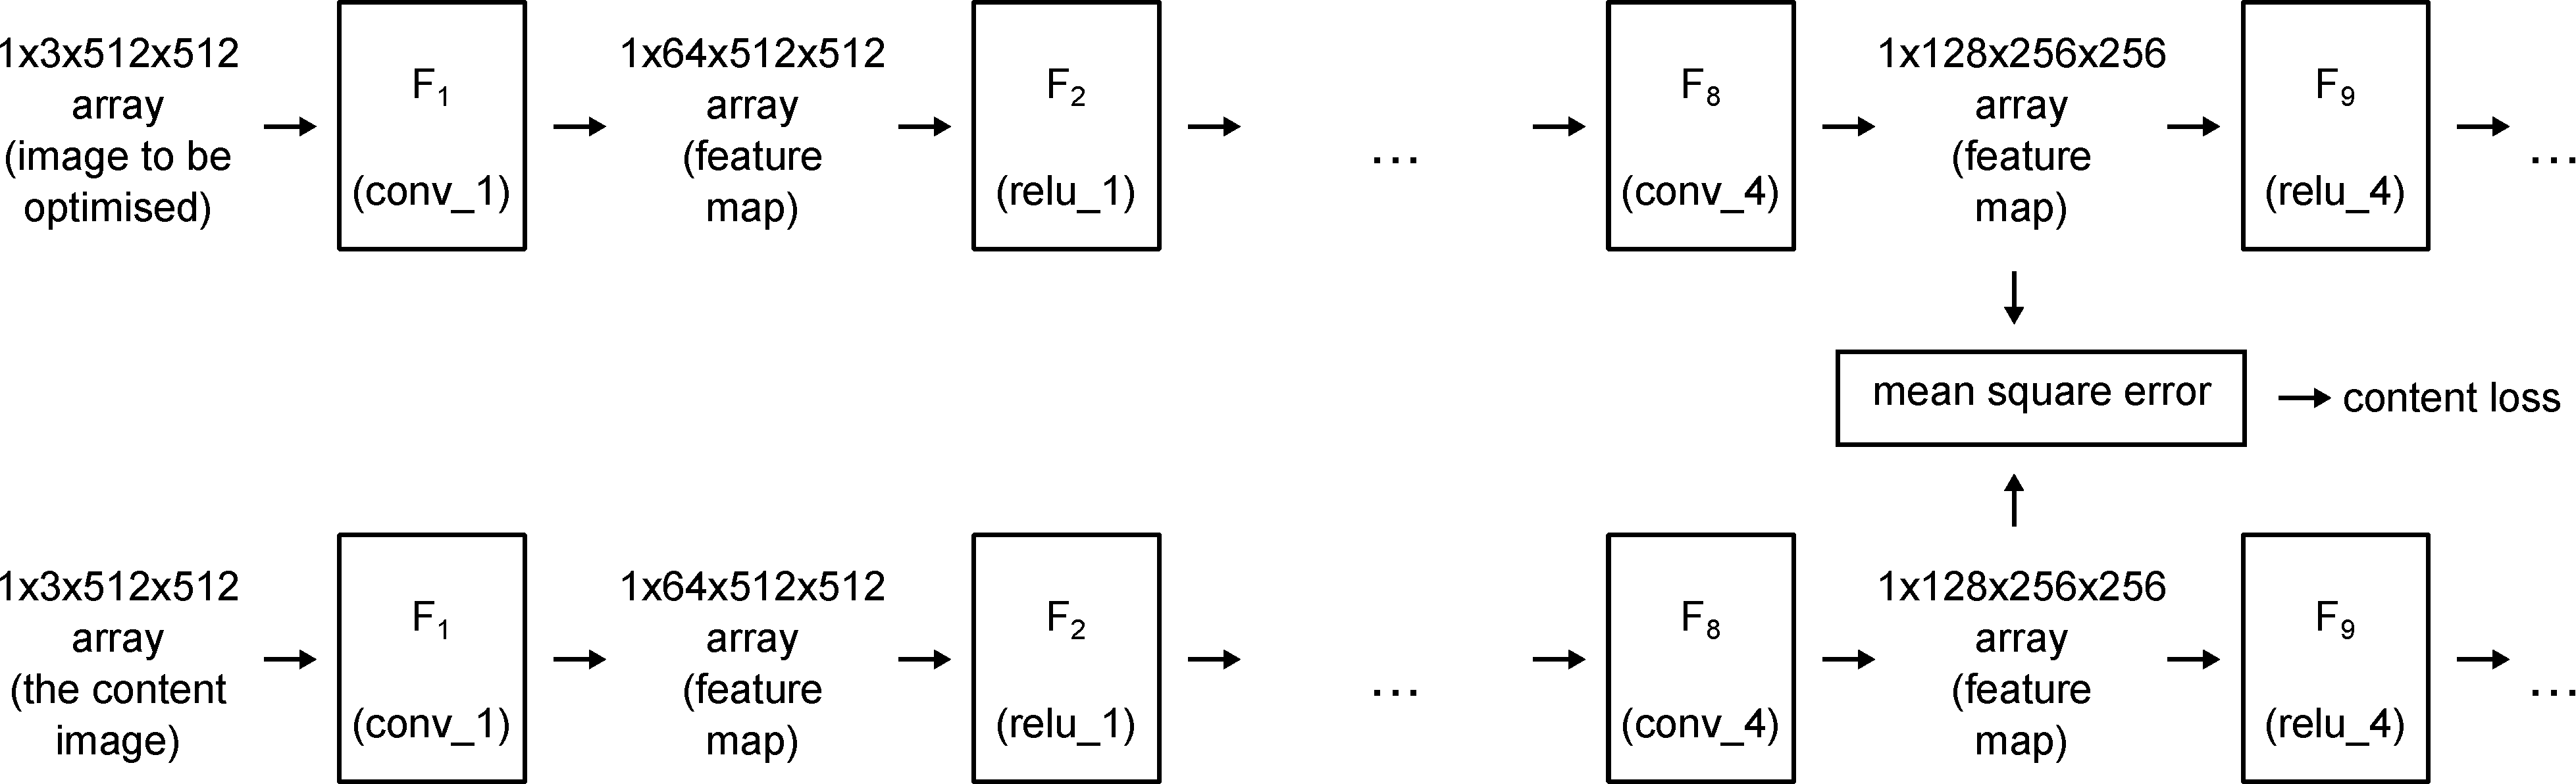
\includegraphics[width=\textwidth]{contentloss.pdf}
\caption{The content loss \label{contentloss}}
\end{figure}

\subsection{Data Set}

\subsubsection {Format and Preparation}

\subsubsection {(Not Really) Time-Series}

\subsubsection {Rationale}

\subsection{Hyperparameters and Experiments}

For the vanilla style-transfer algorithm, there were a few hyper-parameters that 
affected the result.
\begin{itemize}
\item Number of iterations in the optimization. 
We did not have to expriment with different numbers of iterations though.
It was more sensible to run the algorithm for more-than-enough iterations and store the intermediate results.
\item Choice of initial values. Some sensible choices were:
\begin{itemize}
\item White noise.
\item White.
\item Black.
\item The model mean.
\item The content image.
\item The style image.
\item The average of the content image and the style image.
\end{itemize}
\end{itemize}

%\subsubsection{Activation Function}

\subsubsection{Learning Rate}

\subsubsection{Hidden Layer Size}

\subsection{Evaluating Prediction}

\subsubsection{Binarisation and Choice of Loss}

\subsubsection{Amount of Network Reduction}

\subsubsection{Mechanism} 

\subsubsection{Execution}

The program was developed under and are compatible with:
\begin{itemize}
\item Python 3.6
\item PyTorch 1.0.1.post2
\item CentOS 7 x86\_64
\end{itemize}
To run the code, execute shell commands like
\begin{verbatim}
python36 0.py 5000
\end{verbatim}
where 5000 is the number of desired training cycles to reach.
The different hyperparameters will be automatically covered.
The program automatically picks up stored models.
To start fresh, clear the stored models and outputs by
\begin{verbatim}
rm out/*/*.*
\end{verbatim}
but do not remove the directories.


\section{Results and Discussion}

\section{Conclusion and Future Work}

\begin{thebibliography}{8}
\bibitem{nst}
Gatys, L., Ecker, A., \& Bethge, M. (2016). A neural algorithm of artistic style. Journal of Vision, 16(12), 326. doi:10.1167/16.12.326
\bibitem{method}
Gedeon, T.D. and Harris, D. (1991) "Network Reduction Techniques," Proceedings International Conference on Neural Networks Methodologies and Applications, AMSE, San Diego, vol. 1: 119-126. 
\bibitem{prune0}
Penington, Jocelyn \& Dow, R.J.F.. (1988). Neural net pruning—Why and how. Proceedings of the IEEE Conference on Neural Networks. 1. 325 - 333 vol.1. 10.1109/ICNN.1988.23864. 
\bibitem{interp}
Doshi-Velez, F., \& Kim, B. (2017). Towards A Rigorous Science of Interpretable Machine Learning.
\bibitem{example_prune}
Han, S., Mao, H., \& Dally, W.J. (2016). Deep Compression: Compressing Deep Neural Network with Pruning, Trained Quantization and Huffman Coding. CoRR, abs/1510.00149.
\bibitem{example_simplification}
Sun, X., Ren, X., Ma, S., Wei, B., Li, W., \& Wang, H. (2018). Training Simplification and Model Simplification for Deep Learning: A Minimal Effort Back Propagation Method. CoRR, abs/1711.06528.
\bibitem{example_compression}
Cheng, Yu \& Wang, Duo \& Zhou, Pan \& Zhang, Tao. (2017). A Survey of Model Compression and Acceleration for Deep Neural Networks. 
\bibitem{pytorch}
Paszke, A., Gross, S., Chintala, S., Chanan, G., Yang, E., DeVito, Z., Lin, Z., Desmaison, A., Antiga, L., \& Lerer, A. (2017). Automatic differentiation in PyTorch.
\end{thebibliography}
\end{document}

